\documentclass[12pt]{article}

\usepackage{amsmath}
\usepackage[dvips]{graphicx}
\usepackage{psfrag}
\usepackage{fancyhdr}
\usepackage{lastpage}
% \usepackage{natbib}
\usepackage[usenames,dvipsnames]{color}
\usepackage[
  colorlinks=true,
  urlcolor=blue
  ]{hyperref}
%\usepackage{listings}
\usepackage{xspace}
\usepackage{upquote}
\usepackage[T1]{fontenc}
\usepackage{textcomp}

%\lstset{
%    literate={~} {$\sim$}{1}
%}


\topmargin       -0.5truein
\headsep          0.5truein
\headheight       0.0truein
\oddsidemargin   -0.4truein
\evensidemargin  -0.4truein
\textwidth        6.5truein
\textheight       9.0truein

\addtolength{\hoffset}{1.0cm}
\newcommand{\mytilde}{\raise.17ex\hbox{$\scriptstyle\mathtt{\sim}$}}
\pagestyle{fancyplain}
\lhead{}
\chead{\small DFT exercises for Quantum Mobile 2021}
\rhead{}
\cfoot{Page~\thepage~of~\pageref{LastPage}}

% \newcommand{\code}[1]{{\centering \textsc{#1} \\}}
\newcommand{\code}[1]{
\begin{quotation}
  #1 
\end{quotation}
}

\def\QE{\textsc{Quantum ESPRESSO}\xspace}

\def\red#1{\textcolor{red}{#1}}

\begin{document}

\title{
    {\bf DFT exercises for Quantum Mobile} \\
    First-principles calculations of the electronic properties of materials: The case study of bulk sodium chloride
}
\author{
    Davide Grassano,
    Francisco Ramirez,
    Norma Rivano,
    Luca Binci,\\
    Samuel Ponc\'e, 
    Edward Linscott, 
    Iurii Timrov,
    and Nicola Marzari\footnote{This is just the list of the people who did the last significant revision of this material: the content itself has been used in different
    incarnations of this class, initially given at MIT by Nicola Marzari and Gerd
    Ceder, and many have been involved in the versions preceding this one.}\\[4mm]
    {\it \'Ecole Polytechnique F\'ed\'erale de Lausanne (THEOS)}}
\date{February 2021}
  
\maketitle
\tableofcontents
\newpage


%%%%%%%%%%%%%%%%%%%%%%%%%%%%%%%%%%%%%%%%%%%%%%%%%%%%%%%%%%
\section{Introduction}

    There are several popular first-principles codes, and some of them are listed below:

    \begin{itemize}

      \item 
      \QE\, (\href{http://www.quantum-espresso.org/}{http://www.quantum-espresso.org/}).
      This is a DFT plane-wave pseudopotential code. It is distributed under the GPL license. A brief description about this package is given below.

      \item
      ABINIT (\href{http://www.abinit.org/}{http://www.abinit.org/}).
      This is a DFT plane-wave pseudopotential code. It is also distributed under the GPL license.

      \item
      CP2K (\href{https://www.cp2k.org/}{https://www.cp2k.org/}).
      This is a DFT code using the mixed Gaussian and plane-waves approaches. It is also distributed under the GPL license.

      \item
      CPMD (\href{http://www.cpmd.org/}{http://www.cpmd.org/}).
      This is a DFT plane-wave pseudopotential code implementing
      Car-Parrinello molecular dynamics.
      It is also distributed under the GPL license.

      \item
      SIESTA (\href{http://www.uam.es/siesta/}{http://www.uam.es/siesta/}).
      This is a DFT code that uses localized atomic basis sets. 
      It is free for academics.

      \item
      VASP (\href{http://www.vasp.at/}{http://www.vasp.at/}).
      This is a DFT plane-wave pseudopotential code. 
      Available with a moderate cost for academics. %(around \$2000 ? ).

      \item
      WIEN2k (\href{http://www.wien2k.at/}{http://www.wien2k.at/}).
      This is a DFT Full-Potential Linearized Augmented Plane-Wave method (FLAPW).
      FLAPW is the most accurate implementation of DFT, but the slowest.
      Available with  a small cost for academics. % (around \$500).

      \item
      Gaussian (\href{http://www.gaussian.com/}{http://www.gaussian.com/}).
      This is a quantum chemistry code that includes Hartree-Fock (HF) and 
      higher-order correlated electrons approaches.
      Moderate cost for academics. % (around \$3000). 

      \item
      Crystal (\href{http://www.crystal.unito.it/}{http://www.crystal.unito.it/}).
      This is a HF and DFT code.
      Small cost for academics. % (around \$1000).

      \item
      Molpro (\href{http://www.molpro.net/}{http://www.molpro.net/}).
      This is a DFT code.
      Small cost for academics.

    \end{itemize}

    You can find an extended list of codes
    \href{http://nomad-coe.eu/index.php?page=codes}{here}.\\

    In this lab we will use the \QE package \cite{Giannozzi2009quantum}, which is one of the most popular softwares in the condensed matter community. \QE\, is an integrated suite of {\it open-source} computer codes for electronic structure calculations and materials modeling at the nanoscale. \textsc{ESPRESSO} stands for {\it opEn Source Package for Research in Electronic Structure, Simulation, and Optimization}. It is based on density functional theory (DFT), plane waves, and pseudopotentials. It allows one to model structural and electronic properties of materials, vibrational properties (phonons), spectroscopic properties (absorption spectra, electron energy loss spectra, etc.), perform molecular dynamics (Born-Oppenheimer, Car-Parrinello, Langevin) and several other things.

    The PWscf program ({\bf pw.x}) is one of the {\it core} components of \QE\, and it is based on DFT for calculations of the {\it ground state properties} of materials, {\it e.g.} total energy, forces, stress tensor, etc. The rest of this handout will explain how to compute the total energy of a bulk sodium chloride (NaCl) using the PWscf program.
    You can also find many other tutorials for \QE in the
    \href{https://www.quantum-espresso.org/resources/tutorials}{official webpage} of the code and in the
    \href{https://www.materialscloud.org/learn/sections/VLoB41/quantum-espresso-schools}
    {corresponding section} of the Materials Cloud website: especially recommended is the \href{https://www.materialscloud.org/learn/sections/Kr5WSY/summer-school-quantum-espresso-santa-barbara-2009}{hands-on tutorial of Santa Barbara 2009}.
    You can also find \href{https://www.quantum-espresso.org/resources/tutorials}{here}
    a class on atomistic computer modeling of materials (on which this homework is also based) that was taught for 10 years at MIT by Gerd Ceder and Nicola Marzari. 


%%%%%%%%%%%%%%%%%%%%%%%%%%%%%%%%%%%%%%%%%%%%%%%%%%%%%%%%%%
\vspace{6mm}
\subsection{Setting up the work environment}

Computer programs are not always so easy to install and maintain, specially those
designed by scientific researchers.
One of the easiest ways to deal with this issue in the context of learning the use
of a new tool, so that the person learning doesn't need to first start troubleshooting
configuration problems before actually testing the tool itself, is to provide
the necessary codes pre-installed inside of a self-contained working environment
called "Virtual Machine".
This virtual machines can be run using different programs and effectively work
as a "machine inside the machine", with its own libraries, programs and files
and with limited points of contact with the "external device" that is being used
to run it (your physical computer).

To set this up you will first need to download and install
\href{https://www.virtualbox.org/}{VirtualBox}
version 6.1.4 or later: this is the program that we will use to run the virtual
machine. Then you also need to download the virtual machine itself,
\href{https://github.com/marvel-nccr/quantum-mobile/releases/tag/20.03.1}
{Quantum Mobile version 20.03.1},
and import it into Virtualbox (this will occupy 13G of disk space) by going to the "File" menu and choosing "Import Appliance" (use the username "max" and password "moritz", both without the inverted commas).
See Figure \ref{import_vm} for an idea on how VirtualBox looks like and where
to find the "Import Appliance" option; you can also consult the
\href{https://github.com/marvel-nccr/quantum-mobile/wiki/Frequently-Asked-Questions}
{FAQ of Quantum Mobile}
for further information or troubleshooting.
\begin{figure}[h!]
\centering
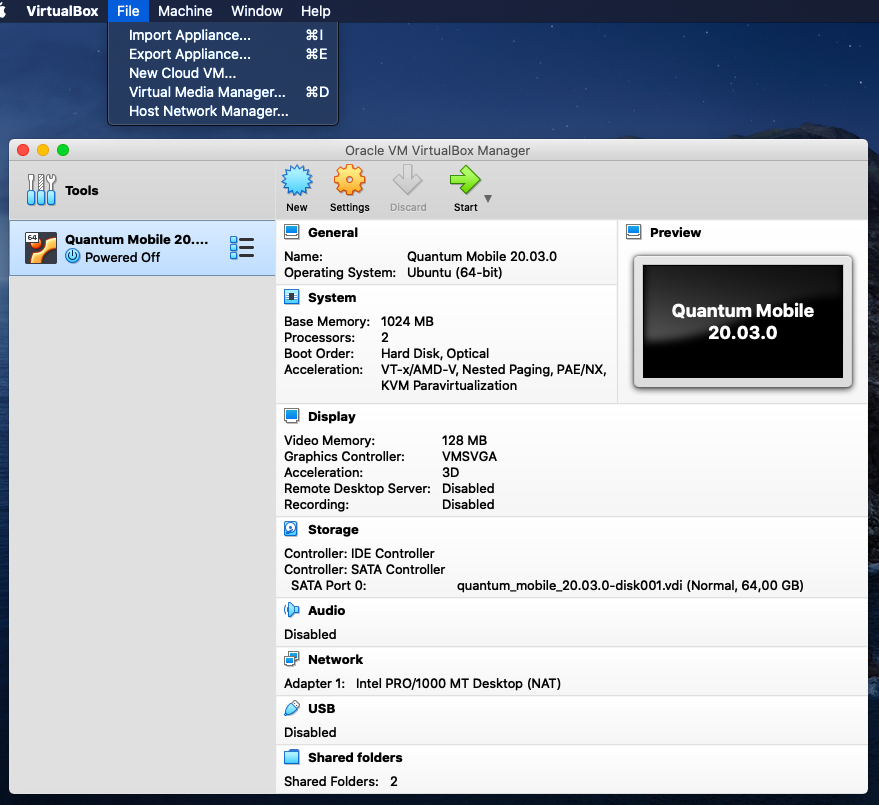
\includegraphics[height=300pt]{import.png}
\caption{VirtualBox interface and "import" option (in MacOS)}
\label{import_vm}
\end{figure}

Now, since the virtual machine does not see the files of the external device, in
order to move files into and out of it we will need to create a "shared folder":
a folder in the external machine that will appear in the internal machine as if
it was an external device (like a pendrive).
To do this, first create a folder on your Desktop called “VM”, then open VirtualBox
and select the Quantum Mobile virtual machine on the left menu and click "Settings"
(make sure you are not currently running the virtual machine).
Click on to the "Shared Folders" section and click on the button to add a new shared
folder (it has a folder and a plus sign in it) to arrive at the menu showed in Figure \ref{shared_folder}.
Select the field "Folder Path", go to the recently created folder "VM" and click on
"Open": the "Folder Name" field should now say "VM" (if it doesn't, write it now),
and you should check the "Auto-mount" checkbox (if you have one).
Finally, in the "Mount Point" field you should write "/home/max/Desktop/SHARED"
and then click the "Ok" button.
The next time you log into your virtual machine, you should see the shared folder
in your desktop and be able to both read the files inside of it and add new
files to it.
\begin{figure}[h!]
\centering
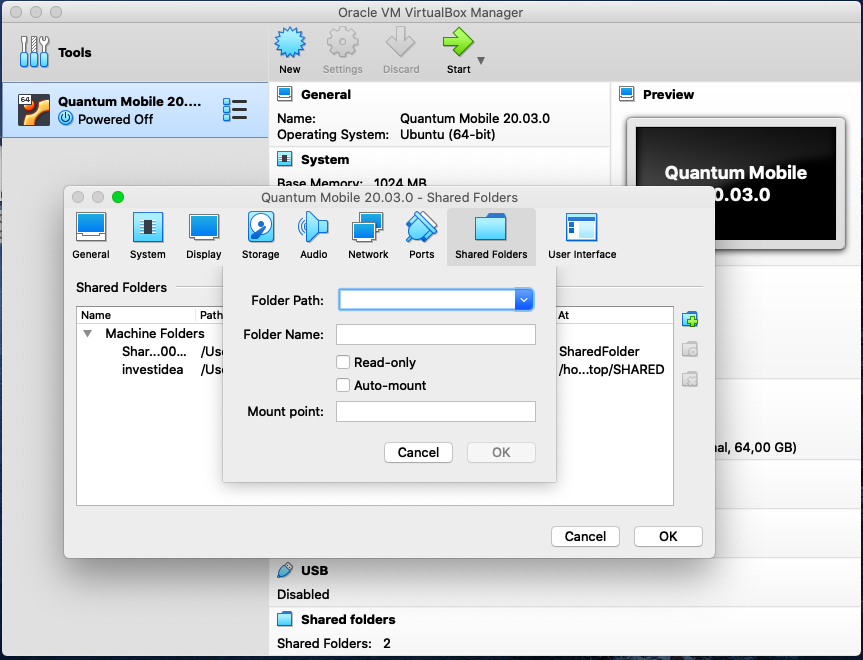
\includegraphics[height=260pt]{shared_folder.png}
\caption{Creating a shared folder}
\label{shared_folder}
\end{figure}

The last configuration you might want to change is the keyboard (in the Virtual
Machine the keyboard is set to the US one). For this you need to go to “Settings”
and choose the language and layout that is appropriate for your own hardware.

As a first step, if you haven't already, you need to download the material by
going to the 
\href{https://github.com/materialscloud-org/learn-fireside}
{github webpagepage of this tutorial}
and clicking on the green "Clone or download" button and then "Download ZIP".
Unzip the learn-fireside-master.zip file and move the generated folder inside of
the shared folder “VM” (if you already had the material, you just need to follow
this last step to make it accessible to the virtual machine).

You can now go into the virtual machine and open a terminal: we will go to the
folder we set up and start working there. We can use the file structure that is
already in place to organize our tests and exercises.
\begin{quotation}
    \noindent
    {\tt max@qmobile:\mytilde\$ cd Desktop/SHARED/learn-fireside-master } \\
    {\tt max@qmobile:\mytilde/Desktop/SHARED/learn-fireside-master\$ ls } \\
    
    (list of folders and files)
\end{quotation}

{\bf Note:} From now on we will start hiding the full path of the current directory in the
commands indications (so we will just use "{\tt max@qmobile:\$}" instead of writing
the full paths like
"{\tt max@qmobile:\mytilde/Desktop/SHARED/learn-fireside-master/(...)\$}").


\vspace{6mm}
\subsection{Input file for the PWscf program}

    First of all we are going to make a basic test to see how PWscf works. 
    To do this, we will first go to the designated directory and then copy the necessary
    files there: the input file for PWscf and folder with the pseudo-potentials.

    \begin{quotation}
        \noindent
        {\tt max@qmobile:\$ cd 0\_initial\_tests } \\
        {\tt max@qmobile:\$ cp ../files/NaCl.scf.in .}\\
        {\tt max@qmobile:\$ cp -r ../files/pseudo . } \\
    \end{quotation}
      
%    To use the scripts provided, you will need to copy the pseudo folder just like
%    that to all the directories in which you want to run these scripts. 
    File NaCl.scf.in contains the input information needed to compute the total energy
    per unit cell of sodium chloride using PWscf, and the directory /pseudo contains the pseudopotential files for sodium (na\_pbesol\_v1.5.uspp.F.UPF) and chlorine (cl\_pbesol\_v1.4.uspp.F.UPF)
    
    If you view the input file, it will look like this:

    \begin{quotation}
        \noindent
        {\tt max@qmobile:\$ less NaCl.scf.in } 
    \end{quotation}
    \begin{verbatim}
    &control
        calculation = 'scf'
        restart_mode = 'from_scratch'
        prefix = 'NaCl'
        tstress = .true.
        tprnfor = .true.
        pseudo_dir = './pseudo/'
        outdir = './tmp/'
    /
    &system
        ibrav = 2
        celldm(1) = 10.5
        nat = 2
        ntyp = 2
        ecutwfc = 20.0
        ecutrho = 160.0
    /
    &electrons
        diagonalization = 'david'
        mixing_mode = 'plain'
        mixing_beta = 0.7
        conv_thr = 1.0d-8
    /
    ATOMIC_SPECIES
        Na  22.990    na_pbesol_v1.5.uspp.F.UPF
        Cl  35.446    cl_pbesol_v1.4.uspp.F.UPF
    ATOMIC_POSITIONS {alat} 
        Na 0.00 0.00 0.00
        Cl 0.50 0.00 0.00
    K_POINTS {automatic}
        2 2 2 0 0 0
    \end{verbatim}

      % \red{All the input parameters are described here:}
    You can find a more detailed description for all the input parameters of pw.x in the
    \href{https://www.quantum-espresso.org/Doc/INPUT\_PW.html\#idm1099}
    {official PW documentation of QE}. 

    \vspace{10mm}
    The most relevant lines for the calculations related to this tutorial are the following:

      \begin{itemize}
        \item
          The line
          \noindent
          \begin{quotation}
          {\tt calculation = 'scf'}
          \end{quotation}
          indicates that this is a self-consistent calculation (SCF) to find the total energy of the system. Other options can be found using the link above.

        \item
          The line
          \begin{quotation}
          {\tt prefix = 'NaCl'}
          \end{quotation}
          is a tag the code uses to identify this calculation. 

        \item
          The line
          \begin{quotation}
          {\tt outdir = './tmp/'}
          \end{quotation}
          indicates the path to the directory to be created by the code, where all temporary files of the code (such as wavefunctions, eigenvalues, etc.) will be written during the execution. 

          {\bf Note:} If you give the same path for {\tt outdir} for two different calculations with the same {\tt prefix}, they will overwrite the temporary files and the calculation will crash. When you run several calculations at the same time, remember to give them different {\tt prefix}, or you can use different temporary directories. 

        \item
          The line
          \begin{quotation}
          {\tt pseudo\_dir = './pseudo/'}
          \end{quotation}
          indicates the path to the place where the pseudopotential file is located. We provide the necessary pseudopotential 
          ({\tt na\_pbesol\_v1.5.uspp.F.UPF} and
          {\tt cl\_pbesol\_v1.4.uspp.F.UPF}) 
          within {\tt LAB2/Examples/pseudo}, just make sure that the path to them is correct in your input file.

        \item
          The line
          \begin{quotation}
          {\tt tstress = .true.}
          \end{quotation}
          indicates that the stress tensor will be computed. 

        \item
          The line
          \begin{quotation}
          {\tt tprnfor = .true.}
          \end{quotation}
          indicates that forces will be computed.

        \item
          The line
          \begin{quotation}
          \noindent
          {\tt ibrav = 2}
          \end{quotation}
          indicates the Bravais-lattice index. In this case {\tt ibrav = 2} means that we are dealing with the face-centered cubic (fcc) primitive unit cell.


        \item
          The line
          \begin{quotation}
          \noindent
          {\tt celldm(1) = 10.5}
          \end{quotation}
          is the value of the lattice parameter in Bohr atomic units.

        \item
          The line
          \begin{quotation}
          \noindent 
          {\tt nat = 2}
          \end{quotation}
          indicates the \textbf{n}umber of \textbf{at}oms in the unit cell.


        \item
          The line
          \begin{quotation}
          \noindent
          {\tt ntyp = 2}
          \end{quotation}
          indicates the \textbf{n}umber of \textbf{typ}es of atoms in the unit cell.  

        \item
          The line
          \begin{quotation}
          \noindent
          {\tt
          ecutwfc = 20.0
          }
          \end{quotation}
          indicates the value of the kinetic-energy cutoff in Rydberg units. This value determines how many plane waves will be used in the expansion of Kohn-Sham wavefunctions during the iterative solution of the Kohn-Sham equations.

        \item
          The lines
          \begin{quotation}
          \noindent
          {\tt ATOMIC\_SPECIES}\\
          {\tt Na  22.990    na\_pbesol\_v1.5.uspp.F.UPF}\\
          {\tt Cl  35.446    cl\_pbesol\_v1.4.uspp.F.UPF}
          \end{quotation}
          indicate the label of the atom, its mass, and the name of the pseudopotential file.


        \item
          The lines
          \begin{quotation}
          \noindent
          {\tt diagonalization = 'david'}\\
          {\tt mixing\_mode = 'plain'}\\
          {\tt mixing\_beta = 0.7}\\
          \end{quotation}
          are the parameters which specify the numerical details for the iterative solution of the Kohn-Sham equation. The final result (e.g. the total energy) must not depend on the value of these parameters. These default values were optimized (for all systems, not only NaCl) and should not be changed. However, there are cases when one has to change these parameters. In this lab, there will be no need to modify these parameters.

        \item
          The line
          \begin{quotation}
          \noindent
          {\tt conv\_thr = 1.0d-8}
          \end{quotation}
          indicates the convergence threshold in Rydberg units during the iterative solution of the Kohn-Sham equation. When this threshold is reached, the calculation will stop.

        \begin{minipage}{\textwidth}
        \item
          The lines
          \begin{quotation}
          \noindent
          {\tt
          ATOMIC\_POSITIONS \{alat\}  \\
            Na 0.00 0.00 0.00 \\
            Cl 0.50 0.00 0.00
          }
          \end{quotation}
          indicate the atomic positions in the unit cell in units of the the lattice parameter ({\tt celldm(1)}).
        \end{minipage}

        \item
          The lines
          \begin{quotation}
          \noindent
          {\tt
          K\_POINTS \{automatic\} \\
           2 2 2 0 0 0
          }
          \end{quotation}
          indicate the $\mathbf{k}$ points sampling of the Brillouin zone. In this case, the automatic $2\times 2\times 2$ $\mathbf{k}$ point sampling will be used using the Monkhorst-Pack procedure \cite{Monkhorst1976special}. The last three numbers indicate that no shift with respect to the center of the Brillouin zone will be made.
      \end{itemize}

These are only some of the possible input settings: the program has many more, for which it usually uses default values when the user doesn't specify them, and the quality of the results obtained will highly depend on the set of parameters used.
We will see some examples in this tutorial of how to calibrate the number of {\tt K\_POINTS} and {\tt ecutwfc}, or how to obtain the relaxed cell dimensions and how to obtain properties of the material by modifying them, but for the rest of the keywords we have already provided a set of values that we know work well for this system and won't be modified (for example, the whole section for {\tt electrons}).

When doing your own research, it might be difficult to know which set of parameters you need to set up, at least as a starting point, to get some decent results.
For this, the
\href{https://www.materialscloud.org/}{Materials Cloud website}
offers a tool called \href{
https://www.materialscloud.org/work/tools/qeinputgenerator}{"Quantum ESPRESSO input generator and structure visualizer"} that will both allow you to check the integrity of the structure you are using and will also make a "first guess" at a good set of keyword values and pseudopotentials that you can use to study the system.
We will now see how you can also check the structure locally with a different program before you start using it to simulate the material.


    %%%%%%%%%%%%%%%%%%%%%%%%%%%%%%%%%%%%%%%%%%%%%%
    \vspace{6mm}
    \subsection{Visualizing the crystal}

    Before you start your first calculation, let us introduce a very useful visualization
    tool called \href{http://www.xcrysden.org/}{XCrySDen}.
    XCrySDen is a crystalline and molecular structure visualization program that allows
    us to visualize our structure and measure its certain properties such as inter atomic
    distances and angles. In the test folder, try typing:

    \code{xcrysden --pwi  NaCl.scf.in}

    which launches the XCrySDen program, indicating that the file that contains the structure to visualize is named "NaCl.scf.in" and has the format of
    a PWscf input ($--$pwi). 
    The program will read the above input file we have seen and visualize it.
    Some useful features are:
    \begin{itemize}
        \item Dimensions pop-up: The first thing you see when you launch the program is 
         to specify if you would like to visualize a 0D, 1D, or 2D structure.
        In this exercise we are visualizing a 3D crystal so choose the {\tt ``do not reduce dimensionality''} option and click {\tt OK}. 
        \item Display tab on top have many features. 
        Choose to display the crystal cell. You can click and rotate the cell and visualize it from 
        different angles. Experiment with it. Although trivial for this example, visualization tools can be very useful for complicated systems.
        \item Go to {\tt Modify} tab and further down into {\tt Number of units drawn}. 
        Play with the numbers there to get a feel of your crystal. 
        \item {\tt Atoms Info, Distance, Angle, Dihedral} tabs below allow you to get info on the atoms or measure distances/angles between atoms.
    \end{itemize}

\begin{figure}[h!]
\centering
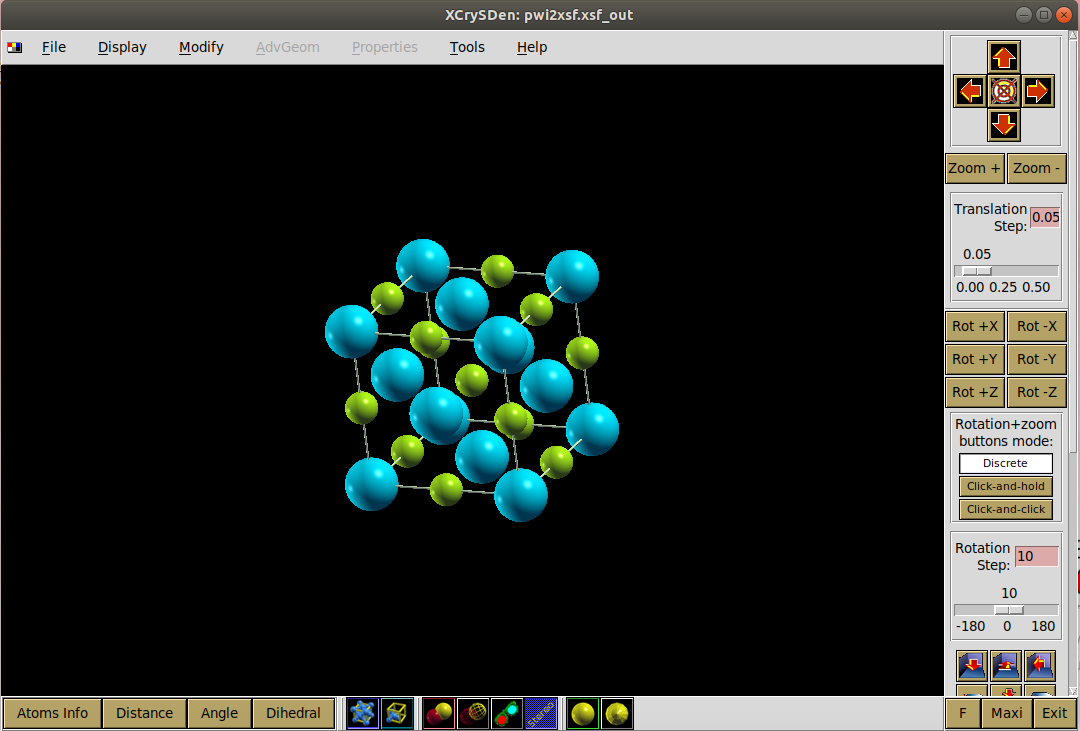
\includegraphics[height=260pt]{xcrysden.png}
\caption{Using XCrySDen to view the NaCl crystal.}
\label{xcrysden}
\end{figure}


    %%%%%%%%%%%%%%%%%%%%%%%%%%%%%%%%%%%%%%%%%%%%%%%%%%%%%%%%%%%%%%%%%%%%%
    \subsection {Running a PWscf example and obtaining the total energy} 

    Now you have seen the crystal structure of bulk NaCl, and we are ready to run our
    first first-principles calculation with PWscf. Close the XCrySDen program and just
    type:
    \code{pw.x < NaCl.scf.in > NaCl.scf.out}

    (we are telling the shell to launch the executable pw.x from a location within the
    {\tt PATH} env variable, pipe the file {\tt NaCl.scf.in} to its {\tt stdin} and pipe
    its {\tt stdout} to the file {\tt NaCl.scf.out}).
    After a few seconds (if everything goes well) you should have in your directory a new
    file called {\tt NaCl.scf.out}.
    This is the output file of your calculation.

    If you view the file {\tt NaCl.scf.out} (you can do su by running {\tt less NaCl.scf.out}, or {\tt vi NaCl.scf.out}, or any other text editor you are comfortable with), you will find that
    in the beginning of the file there is a lot of information which summarizes the
    calculation, such as number of atoms, unit cell size, number of plane waves etc.
    Then you can follow the output file and see how at each iteration the code finds a
    solution with a lower energy. Close to the end, a line containing something like:
    \begin{verbatim}
        !    total energy              =    -128.22614250 Ry
    \end{verbatim}
    will appear.
    This is the final result from the program for the total energy of the unit cell.
    Note that the final occurrence of “total energy” will have an exclamation mark(!)
    next to it, as something to make this line easy to find in a long output file, for
    example by typing, on the terminal, the following:
    \code{grep ! *.out}
    which will search all files terminated by “.out” in the current directory, looking
    for lines that have an exclamation mark in them.

    There is other useful information in the output file. View it again
    {\tt (less NaCl.scf.out)} and go to the end.
    For example, it is written how much CPU and WALL time the PWscf program spends for
    various parts of the calculation:
    \begin{verbatim}
        init_run     :      0.38s CPU      0.76s WALL (       1 calls)
        electrons    :      0.28s CPU      1.46s WALL (       1 calls)
        forces       :      0.03s CPU      0.05s WALL (       1 calls)
        stress       :      0.14s CPU      0.22s WALL (       1 calls)
        .
        .
        .
        PWSCF        :    0.91s CPU        2.88s WALL
    \end{verbatim}

    As you practice with the example exercises, you will get more familiar with the
    output format and all the information written.


    %%%%%%%%%%%%%%%%%%%%%%%%%%%%%%%%%%%%%%%%%%%%%%%%%%%%%%%%%%%%%%%%%%%%%%%%%%%%%%%%
    \subsection{Convergence of the total energy with respect to various input parameters}

      The calculation of various quantities for a given system (e.g. the total energy in this case) must be checked for a convergence with respect to:

      \begin{itemize}
        \item Kinetic-energy cutoff {\tt ecutwfc;}
        \item $\mathbf{k}$ points sampling of the Brillouin zone;
        \item Other parameters (e.g. smearing), which are not needed in our case.
      \end{itemize}

      It is meaningful to speak about the convergence only when we specify the precision. It is not precise to say: "My calculations of the total energy are converged". Instead, it is correct to say: "My calculations of the total energy are converged with a precision, say, of $10^{-3}$~Ry with respect to the cutoff and $\mathbf{k}$ points". This means that if you increase the value of the kinetic-energy cutoff or the density of the $\mathbf{k}$ points sampling, the value of the total energy will not change more than $10^{-3}$~Ry.

      Let us remind some basic concepts in order to understand better about the convergence. A very good explanation of the concepts is given, e.g., in Ref.~\cite{Sholl2011density}. Another excellent book is~\cite{Martin2004electronic}. 


%%%%%%%%%%%%%%%%%%%%%%%%%%%%%%%%%%%%%%%%%%%%%%%%%%%%
\subsubsection {Plane-wave expansion}

    Remember that we are dealing with infinite systems using periodic boundary
    conditions. This means that we can use the Bloch theorem to help us
    to solve the (Schr\"{o}dinger-like) Kohn-Sham equation.
    The Bloch theorem states that the wavefunction can be written in the form:
    %
    \begin{equation}
        \psi_{n, {\bf k}}(\mathbf{r}) = e^{i{\bf k}\cdot{\bf r}} u_{n, {\bf k}}({\bf r}),
        \label{eq:Bloch_def}
    \end{equation}
    %
    where $n$ is the band index, $\mathbf{k}$ is the point in the Brillouin zone,
    $e^{i{\bf k}\cdot{\bf r}}$ is the phase, and $u_{n, {\bf k}}({\bf r})$ is the
    {\it lattice-periodic} part of the wavefunction which can be written as 
    %
    \begin{equation}
        u_{n, {\bf k}}({\bf r}) = \sum_{\bf G} c_{n, \mathbf{k+G}} \, e^{i {\bf G}\cdot{\bf r}} ,
        \label{eq:Bloch_lp}
    \end{equation}
    %
    \begin{equation}
        u_{n, {\bf k}}({\bf r+ R}) \equiv u_{n, {\bf k}}({\bf r}) ,
    \end{equation}
    %
    where $\mathbf{G}$ are the reciprocal lattice vectors, $\mathbf{R}$ is the vector
    of the unit cell in real space, and $c_{n, \mathbf{k+G}}$ are the coefficients of
    the expansion. The sum in Eq.~\eqref{eq:Bloch_lp} runs, in principle, over infinite
    number of the reciprocal lattice vectors ${\bf G}$. In practice, however, one has
    to truncate the sum ({\it plane wave cutoff}).
       
    The basis functions, which we use to make an expansion in Eq.~\eqref{eq:Bloch_lp},
    are {\it plane waves}. They are called "plane waves", because they are surfaces of
    the constant phase and are parallel planes perpendicular to the direction of the
    propagation. The values of $\bf G$ are integer multiples of the three primitive
    lattice vectors, and hence they are compatible with the periodic boundary conditions
    of our direct lattice.

    In actual calculations, we have to limit the plane-wave expansion by specifying the
    plane wave cutoff, which must be given in energy units (such as Rydberg or eV):
    %
    \begin{equation}
    \frac{\hbar^2}{2m} |\mathbf{k}+\mathbf{G}|^2 \leq E_\mathrm{cut} , \quad E_\mathrm{cut} = \frac{\hbar^2}{2m} G^2_\mathrm{cut} ,
    \label{eq:cutoff}
    \end{equation}
    %
    where $\hbar$ is the Planck constant, $m$ is the electron mass, $E_\mathrm{cut}$
    is the cutoff kinetic-energy, and $G_\mathrm{cut}$ is the cutoff reciprocal lattice
    vector.
    Given Eq.~\eqref{eq:cutoff}, Eqs.~\eqref{eq:Bloch_def} and \eqref{eq:Bloch_lp} read:
    %
    \begin{equation}
      \psi_{n, {\bf k}}(\mathbf{r}) = \sum_{|\mathbf{k+G}| \leq G_\mathrm{cut}} c_{n, \mathbf{k+G}} \, e^{i (\mathbf{k+G})\cdot{\bf r}} .
    \end{equation}
    %

    Exercise 1 is designed to test cutoff convergence issues.
    The relevant keyword in the input file is {\tt ecutwfc}.
    You can always choose a higher cutoff in order to increase the precision,
    and this will increase the CPU time of your calculations: in the end,
    you will have to find the right compromise between accuracy and
    efficiency that is needed for your particular system.

    {\bf One always has to perform tests for convergence of the total energy
    (and other quantities of interest) with respect to the kinetic-energy cutoff!}


%%%%%%%%%%%%%%%%%%%%%%%%%%%%%%%%%%%%%%%%%%%%%%%%%%
\subsubsection {$\mathbf{k}$ points sampling of the Brillouin Zone} 

    In order to solve the Kohn-Sham equations, one must calculate various integrals
    in the reciprocal space over $\mathbf{k}$ vectors ($\int d\mathbf{k} (...)$).
    In practice, the integrals over $\mathbf{k}$ vectors are replaced by the summations
    over descrite $\mathbf{k}$ points ($\sum_\mathbf{k} (...)$). Ideally, the number of
    $\mathbf{k}$ points must be infinite, but in practice one has to use a finite number
    and make tests for convergence.

    In the output file of your calculation ({\tt NaCl.scf.out}) you will find something
    like this:
    \begin{verbatim}
        number of k points=    3
                         cart. coord. in units 2pi/alat
          k(    1) = (   0.0000000   0.0000000   0.0000000), wk =   0.2500000
          k(    2) = (   0.5000000  -0.5000000   0.5000000), wk =   1.0000000
          k(    3) = (   0.0000000  -1.0000000   0.0000000), wk =   0.7500000
    \end{verbatim}

    This is a list of the irreducible (non-equivalent) $\mathbf{k}$ points that were
    used to sample the irreducible Brillouin zone. Remember, we specified in the input
    the uniform Monkhorst-Pack $\mathbf{k}$ points sampling of the Brillouin zone:
    $2 \times 2 \times 2 = 8$, but we see here only 3 $\mathbf{k}$ points.
    This is so, because some of these 8 $\mathbf{k}$ points are equivalent due to
    symmetry (give the same Kohn-Sham energy).\footnote{Consider an example of a cube: it has 8 identical corners, so if the original $\mathbf{k}$ point mesh includes 8 corner points,
    it is computationally more convenient (to save CPU time) to calculate the energy using
    one of these corner points and weighing it with the appropriate multiplicity of that
    particular $\mathbf{k}$ point (the corner point of a cube has the multiplicity 8).} 

    Different $\mathbf{k}$ points in the original 8 point mesh have different multiplicities
    in the Brillouin zone of the crystal. The {\bf pw.x} code, using the symmetry, finds these
    multiplicities and lists the non-equivalent $\mathbf{k}$ points and the corresponding
    weights ({\tt wk}). 
    %The weights add up to 2, because we perform unpolarized calculation, and, hence, every Kohn-Sham state is occupied by two electrons due to the Pauli principle (spin degeneracy).

    The list of $\mathbf{k}$ points will be different, if you use a different $\mathbf{k}$
    point mesh ($4\times 4 \times 4$, $6\times 6 \times 6$, $8\times 8 \times 8$, etc.). {\bf One always has to
    perform tests for convergence of the total energy (and other quantities of interest)
    with respect to the number of $\mathbf{k}$ points!}

%%%%%%%%%%%%%%%%%%%%%%%%%%%%%%%%%%%%%%%%%%%%%%%%%%%%%%%%%%%%%%%%%%%%%%%%%%%%%%%%
\newpage
\subsection{Using bash scripts to run PWscf multiple times}

    In order to check the numerical convergence of your calculations with respect to
    kinetic-energy cutoff and the number of $\mathbf{k}$ points, you will have to run
    PWscf multiple times with different values for those parameters.
    Of course you may create a new input file for every set of parameters, but there are faster automatized ways of doing this.
    We would like to introduce to you one of them: {\it bash scripting}.

    You can either write a bash script by yourself or use the one from the example provided
    in {\tt learn-fireside-master/files/script.sh}. 
    The script looks like this:

    \begin{verbatim}
    #!/usr/bin/env bash

    # Input data:
    LISTA="10.5"      # List of values of lattice parameter to try
    LISTECUT="20 30"  # List of plane-wave cutoffs to try
    LISTK="2 4"       # List of number of k-points per dimension to try

    # Files of interest:
    TMP_DIR="./tmp"          # where temporary data will be stored
    PSEUDO_DIR="./pseudo"    # where pseudopotentials are stored
    OUT_DIR="./Test_script"  # where input and output will be
                                  # created once the script runs.

    PW_LAUNCH='pw.x'         # This is QE executable file.

    # Security checks:
    if [ ! -d $TMP_DIR ]; then
        mkdir $TMP_DIR
    fi

    if [ ! -d $OUT_DIR ]; then
        mkdir $OUT_DIR
    fi

    SAVE="SAVE.txt"

    echo "#   a(bohr)  ecut (Ry)  num_kpt      E_tot (Ry)    F_x Na    F_y Na  ...  
              ...  F_z Na    F_x Cl    F_y Cl    F_z Cl (Ry/au)" >> $SAVE
    # Start loops on plane-wave cutoffs, k-point grids, and lattice constants:
    for ecut in $LISTECUT; do
        for k in $LISTK; do
            for a in $LISTA; do

            INPUT="NaCl.scf.a=$a.ecut=$ecut.k=$k.in"
            OUTPUT="NaCl.scf.a=$a.ecut=$ecut.k=$k.out"
            echo 'Doing ecut, k, a: ' $ecut $k $a
            # Create new input file:
    cat > $OUT_DIR/$INPUT << EOF
            &control
                calculation = 'scf'
                restart_mode = 'from_scratch'
                prefix = 'NaCl.$a.$ecut.$k'
                tstress = .true.
                tprnfor = .true.
                pseudo_dir = '$PSEUDO_DIR'
                outdir='$TMP_DIR'
            /
            &system
                ibrav = 2
                celldm(1) = $a
                nat = 2
                ntyp = 2
                ecutwfc = $ecut
            /
            &electrons
                diagonalization = 'david'
                mixing_mode = 'plain'
                mixing_beta = 0.7
                conv_thr = 1.0d-8
            /
            ATOMIC_SPECIES
                Na  22.990    na_pbesol_v1.5.uspp.F.UPF
                Cl  35.446    cl_pbesol_v1.4.uspp.F.UPF
            ATOMIC_POSITIONS {alat} 
                Na 0.00 0.00 0.00
                Cl 0.50 0.00 0.00
            K_POINTS {automatic}
                $k $k $k  0 0 0
    EOF

            # Run PWscf to create new output file:
            $PW_LAUNCH < $OUT_DIR/$INPUT > $OUT_DIR/$OUTPUT

            # E_TOT=$(cat $OUT_DIR/$OUTPUT | grep ! | tr -dc '[0-9]\.\-\n')
            # NKPT=$(cat $OUT_DIR/$OUTPUT | grep "number of k points=" |
               tr -dc '[0-9]\.\-\n')
            # F1_x=$(cat $OUT_DIR/$OUTPUT | grep " atom    1 type  1   force" |
               cut -d= -f2 | tr -dc '[0-9]\.\-\n ' | tr -s ' ' | cut -d' ' -f2)
            # F1_y=$(cat $OUT_DIR/$OUTPUT | grep " atom    1 type  1   force" |
               cut -d= -f2 | tr -dc '[0-9]\.\-\n ' | tr -s ' ' | cut -d' ' -f3)
            # F1_z=$(cat $OUT_DIR/$OUTPUT | grep " atom    1 type  1   force" |
               cut -d= -f2 | tr -dc '[0-9]\.\-\n ' | tr -s ' ' | cut -d' ' -f4)
            # F2_x=$(cat $OUT_DIR/$OUTPUT | grep " atom    2 type  2   force" |
               cut -d= -f2 | tr -dc '[0-9]\.\-\n ' | tr -s ' ' | cut -d' ' -f2)
            # F2_y=$(cat $OUT_DIR/$OUTPUT | grep " atom    2 type  2   force" |
               cut -d= -f2 | tr -dc '[0-9]\.\-\n ' | tr -s ' ' | cut -d' ' -f3)
            # F2_z=$(cat $OUT_DIR/$OUTPUT | grep " atom    2 type  2   force" |
               cut -d= -f2 | tr -dc '[0-9]\.\-\n ' | tr -s ' ' | cut -d' ' -f4)

            # echo "`printf "%11.4f %10.1f %8d %15.6f %9.6f %9.6f %9.6f %9.6f
               %9.6f %9.6f" $a $ecut $NKPT $E_TOT $F1_z $F1_y $F1_z
               $F2_x $F2_y $F2_z`" >> $SAVE

            # Finish loops on plane-wave cutoffs, k-point grids, and lattice constants:
            done
        done
    done

    rm -r $TMP_DIR/*

    echo -e "\n" >> $SAVE

    \end{verbatim}
    
    You can see that there are three lists of input parameters that will be created in
    order:
    \begin{verbatim}
        LISTA="10.5"       
        LISTECUT="20 30"    
        LISTK="2 4"         
    \end{verbatim}
    The bash script will loop over these values to perform  (in this case) four
    different calculations automatically, without having to change the input files
    by hand.
    
    You can run the script by doing:\footnote{You can use instead \code{hohup ./script.sh $\&$} where the {\tt \&} symbol at the end of the line allows you to keep using the terminal without having to wait for the work to finish, and the {\tt nohup} part allows
    the program to keep running even if you close the terminal in the computer.}

    \code{./script.sh}

    At the end you will find several output files in your output directory. Go in the output directory "Test\_script" and type {\tt ll} to get a list of the produced files.

    In order to solve the exercises without having to manually create and run all the
    inputs, we suggest that you try to modify the above script accordingly to adapt
    it to the different calculations you need.

%%%%%%%%%%%%%%%%%%%%%%%%%%%%%%%%%%%%%%%%%%%%%%%%%%%%%%%%%%%%%%%%%%%%%%%%%%%%%%%%
\newpage
\subsection{Running PWscf on the VM using multiple CPUs}
    For most of the exercises that you will have to do, executing \texttt{pw.x} with only
    one core will be enough to finish them in a matter of a few minutes.
    Nevertheless, the last exercises will be more demanding than the others, as it requires
    to run relax calculations on a supercell.
    Because of this, it is advisable to increase the number of CPUs
    assigned to the VM (if you have a fast computer).
    In order to do so you have to:
    \begin{itemize}
      \item Shutdown the VM (full shut-down).
      \item Select the VM in the VBox interface
      \item Click on 'Settings' 
\includegraphics[height=20pt]{settings.png}
      \item Click on 'System' in the left sidebar 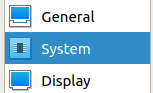
\includegraphics[height=40pt]{system.png}
      \item Click on 'Processor' in the tab bar and change  the number of CPUs (we recommend half of the maximum value or before you reach the red part of the slider bar). If you can't change this it means the VM was not totally turned off. \\
      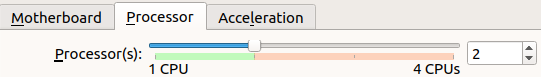
\includegraphics[height=40pt]{processors.png}
      \item Press 'Ok' to save the changes
    \end{itemize}

    \vspace{6mm}
    In order to make use of having multiple CPUs you will need to launch the
    calculation using 'mpirun':\footnote{Depending on the environment setup, the command 'mpirun' could be different (e.g.  'srun').}
    \begin{itemize}
      \item From the command line:
            \code{mpirun -np 2 pw.x $<$ input\_name $>$ output\_name}
      where 2 is the number of CPUs (this number can be larger than 2 of course, but it cannot be larger than the total number of CPUs allocated to the Quantum Mobile, shown on the image above).

      \item From a script: locate the line that sets the executable
            \code{PW\_LAUNCH $=$ "pw.x"}
            And change it to:
            \code{PW\_LAUNCH $=$ "mpirun -np 2 pw.x"}

    \end{itemize}

    With a small amount of CPU, the improvement you should experience in
    run time should be linear (eg. twice the CPUs $\approx$ half the time).
    Be aware that this is true for long calculations, as the serial part of
    the code execution should be negligible compared to the parallel one.
    For shorter calculations the scaling will be different.


%%%%%%%%%%%%%%%%%%%%%%%%%%%%%%%%%%%%%%%%%%%%%%%%%%%%%%%%%%%%%%%%%%%%%%%%%%%%%%%%
\newpage
\section{Exercise examples using \QE}

In order to do the following exercises, you will have to run several PWscf (pw.x)
calculations.
We suggest that you use the folder structure that is already in place in the
file you downloaded from the github page.
Ultimately, you can organize directories for saving the output runs in any way
you like, but you might need to do some modifications in the bash scripts provided.

\vspace{6mm}
\subsection{Exercise 1: Convergence tests for input parameters}


\vspace{6mm}
\subsubsection*{A) Convergence of {\it total (absolute) energies} with respect to cutoff energies}

In exercise 1.1 we will check the convergence of the total energy with respect to the
kinetic-energy cutoff: for this you need to run scf calculations of bulk NaCl for
different values of this parameter and obtain the total energy.
A good range to try is 10-150 Ry, doing calculations at increments of 10 Ry: in order
to do this using the {\tt script.sh}, modify the content of {\tt LISTECUT} so that different
numbers are included.
When changing the cutoff, make sure to keep the other variables (lattice constant,
$\mathbf{k}$ points mesh, etc.) fixed and to record them: this means that you should
set {\tt LISTK} to only one value ({\tt '4'} if you are using the provided bash script).
Or if you are preparing your input files manually, keep the $\mathbf{k}$ point mesh
always as 4 4 4  0 0~0.

Record and plot your final results.
What is the smallest value of the cutoff (parameter "ecutwfc") at which the total energy is converged with the accuracy of 5 meV/atom?
Note that PWscf calculates the total energy per unit cell (not per atom) in atomic units
(so Rydberg instead of eV).

{\bf Note:} You should see that as you increase the value of the cutoff energy, and
thus include more basis functions, the energy decreases in a monotonical way.
This is because the increase in basis functions available can only improve the accuracy
of the candidate for the wavefunction of the system (worst case scenario, you just end
up using the combination of basis that when you had a lower cutoff) and therefore the
energy can only be equal or lower.


\vspace{6mm}
\subsubsection*{B) Convergence of {\it forces} with respect to cutoff energies}

In some cases, we are interested in quantities other than energies, e.g. forces acting on atoms.
In the previous exercise, the forces on Na and Cl were zero in the $x$, $y$, and $z$
directions because of symmetry.
(Forces are written at the end of the output file NaCl.scf.out for each atom in the unit cell, you can check that they are indeed zero.)
Therefore now we want to create forces by displacing a Cl (or Na) atom by +0.05
(fractional coordinates) e.g. in the $z$ direction.
To do this, we need to edit the $z$ coordinate of the Cl (or Na) atom in the input file.
After editing the script "script.sh", the corresponding lines will look like this:
%\vspace{6mm}
\newpage
%\begin{minipage}{\textwidth}
\begin{verbatim}
        ATOMIC_POSITIONS {alat}
        Na  0.00 0.00 0.00
        Cl  0.50 0.00 0.05
\end{verbatim}
%\end{minipage}

\vspace{2mm}
Now put {\tt '30'} in {\tt LISTECUT} so that the cutoff is 30 Ry, and put {\tt '4'}
in {\tt LISTK} so that the $\mathbf{k}$~point grid is $4 \times 4 \times 4$.
The forces will appear in the output file after the total energies.
It will look something like this:
\begin{verbatim}
    Forces acting on atoms (cartesian axes, Ry/au):

    atom    1 type  1   force =     0.00000000    0.00000000    0.02522765
    atom    2 type  2   force =    -0.00000000   -0.00000000   -0.02522765

    Total force =     0.035677     Total SCF correction =     0.000032
\end{verbatim}
(You can also notice that by displacing an atom we are lowering the symmetry of
the system, hence more irreducible kpoints will be present with respect with the
previous calculations.)

Now test the convergence of forces with respect to cutoff while keeping other
parameters fixed.
Reach the convergence of the total force to within 10 meV/\AA \, (again, notice that PWscf
gives forces in Ry/Bohr).
Record relevant parameters. Use the $\mathbf{k}$ points mesh fixed to
$4 \times 4 \times 4$ centered at the Brillouin zone.
Plot and record your results.

Hint: 1 meV/\AA \, = $4 \times 10^{-5}$ Ry/Bohr.


\vspace{6mm}
\subsubsection*{C) Convergence of the {\it total (absolute) energies} with
respect to the size of the $\mathbf{k}$ points mesh}

In this exercise you need to convergence the total energy with with respect to the
size of the $\mathbf{k}$ point grid.
For each mesh, record the number of the $\mathbf{k}$ points in the irreducible wedge
of the first Brillouin zone (\red{not the size of the grid}): this gives a measure of
how long your calculation will take, as calculations scale linearly with the number of
$\mathbf{k}$ points.
When changing the size of the $\mathbf{k}$ points mesh, make sure to keep all other
input parameters fixed (lattice constant, energy cutoff, etc.): in particular, you
need to use the converged cutoff energy found in exercise 1.

In order to increase the size of the $\mathbf{k}$ point grid, edit the script and change
the values in {\tt LISTK}, putting {\tt '2 4 6 8'} instead of {\tt '4'}.
Submit the calculations using your modified script, and record the total energies for the following grids
$2 \times 2 \times 2$, $4 \times 4 \times 4$, $6 \times 6 \times 6$ and
$8 \times 8 \times 8$ (or even denser grids, if you find it necessary).
To get the number of irreducible $\mathbf{k}$ points, you can search in the output file
for the following:
\begin{verbatim}
    number of k points=    16
\end{verbatim}

{\bf Note:} Contrary to what happen with the cutoff energy, you may notice that now
the energy is not a monotonically decreasing function of the $\mathbf{k}$ point grid.
This is because changing the $\mathbf{k}$ point grid does not affect the wavefunction
directly, but through increasing the precision with which the DFT problem is solved.
The total energy is not variational with respect to $\mathbf{k}$, hence it is not a monotonic function with respect to the number of $\mathbf{k}$ points.

\vspace{6mm}
\subsubsection*{D) Convergence of {\it forces} with respect to the size of the
$\mathbf{k}$ points mesh}

Now you need to perform a test for convergence of forces with respect to the number of $\mathbf{k}$ points.
Like in exercise 2, in order to calculate the force acting on a Na (or Cl) atom, you need to displace it by $+0.05$ in the $z$ direction (in fractional coordinates).
But this time, like in exercise 3, you will increase the density of the $\mathbf{k}$
point grid by modifying the script and change the values in {\tt LISTK}, putting
{\tt '6 8'} (or even denser if needed) instead of {\tt '4'} and recording the forces.
Remember to keep all other parameters fixed and record all of the relevant ones
(lattice parameter, energy cutoff, etc.).
Reach the convergence on forces to within around 10 meV/\AA.

\vspace{6mm}
\subsubsection*{E) Convergence of the {\it total energy differences} with respect to energy cutoff}

In practice only energy differences have physical meaning, as opposed to absolute energy
scales, which can be arbitrarily shifted.
Therefore, the final convergence test that we will see here is the one for the total
energy difference between two crystals at different lattice parameters, as a function
of cutoff.
For example, you could calculate the energy of NaCl at the experimental lattice distance
of 5.640 Angstrom, and then calculate the energy using another value close to it (5.644 Angstrom, for example), take the difference between the two energies, and repeat this
process for many energy cutoffs.
As always, make sure to keep all other input parameters (lattice constant, $\mathbf{k}$
points mesh, etc.) fixed while changing the energy cutoff by putting only one value in
the lists of the script that are not relevant for this test.
Record all relevant parameters such as the lattice constant, $\mathbf{k}$ points mesh, etc.
Keep increasing the energy cutoff until you reach the convergence to around 5 meV/atom.

\vspace{6mm}
\subsection{Exercise 2: Determination of the {\it equilibrium lattice parameter}
and {\it bulk modulus}}

We will now use the program to make a series of calculations that will allow us to
calculate the properties mentioned for the material we have been testing.
For this, you will use the energy cutoff and $\mathbf{k}$ points mesh which you determined
for the force and energy difference calculations.
Usually, one is interested in quantities such as forces and energy differences and
that is why we made the convergence test with those quantities.
But more in general, to be absolutely safe, one should test the convergence of the quantity
one is interested in (lattice parameter and bulk modulus in this case) with respect to the
energy cutoff and $\mathbf{k}$ points mesh (and other parameters, which we don't have for
our system (e.g. smearing)).
We are not going to do it like that in this tutorial but it is something you should
take into account when working on your own research project.

This exercise is divided in the following steps:

\begin{itemize}

    \item[A)]
    Calculate the equilibrium lattice parameter of NaCl and compare this theoretical
    (computed) value $a_0^{theor}$ with the experimental equilibrium lattice parameter
    $a_0^{exp} = 5.640$~\AA. Make sure to record all the relevant input parameters
    of the calculations (energy cutoff, $\mathbf{k}$ points mesh, etc.).

    \item[B)]
    Calculate the bulk modulus $B$ of NaCl.
    The bulk modulus is a measure of the stiffness of a material and it is defined
    as $$ B = - V_0 \frac{\partial P}{\partial V}, $$ where $P$ is the pressure on
    the material, $V$ is its volume, and $V_0$ is its equilibrium volume.
    Knowing that $P=-\partial{E}/\partial{V}$, you need first to derive from the previous
    equations the direct relationship between the magnitude to compute and the results
    obtainable through the calculations: energies per unit cell for different cell
    sizes/volumes. 

    \item[C)]
    Calculate the bulk modulus $B$ of NaCl using the third-order Birch-Murnaghan
    isothermal equation of state.
    We suggest to use the interactive {\bf ev.x} program provided with
    \QE, which contains the implementation of this equation.
    In the input file for ev.x you have to provide two columns for the case of an FCC
    lattice: the first one contains the lattice parameter and the second one the total
    energy obtained.
    The fitting function is labeled as "birch2".

\end{itemize}
\vspace{6mm}

The first item of this exercise requires you to calculate the total energy as a function
of the cell volume, so at the end of it you will have a relationship between some important
state variables such as volume and pressure, i.e. which volume corresponds to which pressure,
for each data point you have. 
Such information is very significant in solid state physics, it helps us identify different
phases of matter and phase transitions between them, as each phase of matter has a unique
response to compression.

Ultimately, if we could recast this relationship into a mathematical function instead of
data point-by-data point analysis, we would gain more predictive power about the properties
of each phase.
In first approximation we could approximate the energy vs the volume to the second order
of Taylor expansion and use the relation $P=-\partial{E} / \partial{V}$ to calculate $P(V)$.
A better approach would be to use a more refined \textit{Equation of State} to describe
the relationship between these variables, as proposed in items b and c.
There are several suggestions for the shape of this function, but the chosen one for
this example is the {\it third-order Birch-Murnaghan isothermal equation of state}:
%
\begin{equation}
    P(V) = \frac{3B_0}{2}
    \left[ 
        \left(\frac{V_0}{V}\right)^\frac{7}{3} - 
        \left(\frac{V_0}{V}\right)^\frac{5}{3}
    \right] 
    \left\{
        1 +
        \frac{3}{4}(B^\prime_0 - 4)
        \left[
        \left(\frac{V_0}{V}\right)^\frac{2}{3} - 1
        \right]
    \right\} , 
\end{equation}
%
where $P$ is the pressure, $V_0$ is the equilibrium volume, $V$ is the deformed volume,
$B_0$ is the bulk modulus, $B'_0$ is the derivative of the bulk modulus with respect to
pressure. 
Integration of this pressure expression with volume gives us the energy versus volume
relationship as below:
% 
\begin{equation}
    E(V) = E_0 +
    \frac{9V_0B_0}{16}
    \left\{
        \left[ \left(\frac{V_0}{V}\right)^\frac{2}{3} - 1 \right]^3 B'_0 +
        \left[ \left(\frac{V_0}{V}\right)^\frac{2}{3} - 1 \right]^2
        \left[ 6 - 4 \left(\frac{V_0}{V}\right)^\frac{2}{3} \right]
    \right\}.
\end{equation}
% 
We can make several calculations at different cell volumes and obtain energies.
By fitting the above equation to the data we have, we can obtain the values for
equilibrium volume, bulk modulus and bulk modulus derivative.
Thus, with these few parameters we computed, we can reveal the energy vs. volume or
pressure vs. volume relationship for a wide range of volume.

%You might assume that such approach is of little use in our age of very powerful computers,
%as one could obtain the $E(V)$ or $P(V)$ relationship of each material by simply running the
%calculation at more points and calculating the stress tensor, therefore pressure from
%first-principles.
%However, we need to come back to the issue of numerical convergence again: stress tensor
%often requires many plane waves to converge, for most materials it requires several times
%the plane wave cutoff required for energy differences.
%\QE CPU time scales as $E_{cut}^{(3/2)}$, therefore you can see that calculating pressure
%{\it ab initio} quickly gets too computationally demanding. That is why it is still a
%common method to obtain the pressure at given volume from an equation of state fit.

\QE is shipped with a small program that does the fitting we have mentioned above, given the energy vs. volume data. This program is called \textbf{ev.x}.
The program {\bf ev.x} works interactively: it expects that you specify units
('Ang' or 'ANG'  or 'ang' indicates Angstroms, while any other input will default
to atomic units (Bohr)), the type of Bravais lattice that you used, the type of the equation
of state that you want to use for a fit, and a data file where the first column is the
lattice parameter (or volume in case of 'noncubic'$\equiv$'hex') and second is the energy
in Ry.



\vspace{6mm}
\subsection{Exercise 3: Determination of the {\it elastic constants}}

This is the second and last application to material properties that we will show
in this tutorial.
For this, it will be necessary to make alterations in the cell, resulting from the
application of certain "strains" that respect certain symmetries, and for which it
will be convenient to use the conventional unit cell containing 8 atoms and the
orthorombic ({\tt ibrav=8}) and monoclinic ({\tt ibrav=12}) Bravais lattices
(For a list of all possible indications of {\tt ibrav} please click
\href{https://www.quantum-espresso.org/Doc/INPUT_PW.html#idm199}{here}).
We suggest to you to read Ref.~\cite{Mehl1994first} in order to learn about the first
principles calculations of the elastic constants.

For a demonstration on how to construct an orthorhombic cell, let us assume that the unit
cell we aim to construct has the following lattice vectors (in cartesian coordinates,
and in Bohr):
%
\begin{quotation}
v1=(a,0,0), v2=(0,b,0), v3=(0,0,c)
\end{quotation}
%
meaning that it is \textbf{a} Bohr long in x direction, \textbf{b} Bohr long in y,
and \textbf{c} Bohr long in z.
We can specify this cell in the following way:
%
\begin{quotation}
{\tt ibrav = 8 \\
celldm(1) = a \\
celldm(2) = b/a \\
celldm(3) = c/a}
\end{quotation}
%
where instead of {\tt b/a} type of expression, you should put the result of the division,
not the expression itself.

On the other hand, the monoclinic cell has two 90$^\circ$ angles and one that is
different from 90$^\circ$. The convention that \QE\, adopts by {\tt ibrav=12} is
such that the unique, non-90$^\circ$ angle is $\gamma$, the one between v1 and v2,
where:
% 
\begin{quotation}
v1=(a,0,0), v2=(b$\times cos(\gamma)$,b$\times sin(\gamma)$,0), v3=(0,0,c)
\end{quotation}
%
where our first vector is \textbf{a} Bohr long in x direction, our second vector is
$\mathbf{b}$ Bohr long but lays in $x-y$ plane, with components both on x and y with
a dependence on angle $\gamma$, and our third vector is \textbf{c} Bohr long in z axis.
We can specify this cell in the following way:
\begin{quotation}
    {\tt ibrav = 12} \\
    {\tt celldm(1) = a }\\
    {\tt celldm(2) = b/a }\\
    {\tt celldm(3) = c/a } \\
    {\tt celldm(4) = cos($\gamma$) }
\end{quotation}
%
and again, replace the expressions with the numerical values, including the cosine.

IMPORTANT: although we are using different lattices and cell, you can use the converged
parameters that you estimated in exercise 1.
In principle, you should need less $k$ points with the conventional supercell to get to
convergence; in your own research you should repeat the convergence tests for these new
lattices and cell.

Upon the application of the strain, it may happen that not all atomic positions in the
cell are fixed by symmetry, as there is more than one basis element (i.e. a sodium and
chlorine atom). 
Therefore, when we apply the strain one of these atoms could move to another relative
position than the initial (1/2, 0, 0) and lower the total energy of the cell. 
Hence, to calculate the elastic constant of this system, we should allow the cell to
relax the atoms to their equilibrium positions instead of fixing them to relative positions,
which can be done very easily with \QE.
The necessary modification is changing the {\tt calculation} variable in {\tt control} namelist, from {\tt scf} to {\tt relax}
\begin{quotation}
{\tt 
    calculation="relax"
}
\end{quotation}

And now since we will move the ions we will need a new namelist called {\tt ions}:

~~~~~~~{\tt \&ions} 
~~~~~~~{\tt    / }


Note that you can place this new namelist after the electrons namelist (after the slash)
and since we will only use default parameters you do not need to specify anything in this
namelist. 
Therefore we only declare the namelist with the \&, and close it with a slash right away. 
          
You will compute the energetics of deformation, and fit the resulting energy curves in two
different ways [A] and [B].
You can then compare your results with the \href{https://doi.org/10.1016/S0022-3697(72)80468-2}{experimental data}.


\begin{itemize}

\item[A)]
Compute $C_{11}-C_{12}$ using the orthorombic ({\tt ibrav=8}) Bravais lattice, and using
the relation $B = \frac{1}{3} (C_{11} + 2 C_{12})$ determine the elastic constants $C_{11}$
and $C_{12}$. Then compute $C_{44}$ using the monoclinic ({\tt ibrav=12}) Bravais lattice.

\item[B)]
Compute $C_{11}-C_{12}$ using {\tt ibrav=0} and specifying the card {\tt CELL\_PARAMETERS},
and then use the relation for $B$ (as above) to determine the elastic constants $C_{11}$ and
$C_{12}$. Compute $C_{44}$ using {\tt ibrav=0} too.

\end{itemize}



%%%%%%%%%%%%%%%%%%%%%%%%%%%%%%%%%%%%%%%%%%%%%%%%%%%%%%%%%%%%%%%%%%%%%%%%%%%%%%%%
\newpage
\section{FAQ}

\begin{itemize}

    \item
    {\bf How precisely do I need to compute the lattice parameter?}

    Lattice parameters are typically reported in papers to within 0.01 \AA.
    However, there are cases when higher precision is required; this is {\em not} 
    one of them.

    \item
    {\bf Is the total energy higher when you move an atom (the force calculations) 
    with respect to the equilibrium position?}

    Yes. Remember: at equilibrium the energy is the lowest.
    Equilibrium for this structure has a Na atom at (0, 0, 0) and Cl at
    (0.50, 0.0, 0.0).
    As a side note the forces will give you an idea of how far the system is from
    equilibrium (they tell you which direction the atoms ``want" to move).
    The stresses tell you which direction the cell parameters ``want" to change to
    reach equilibrium.

    \item
    {\bf My energy versus lattice constant plot is jagged.}

    There are a number of solutions to this; the easiest is to raise the energy
    cutoff.

    \item
    {\bf How is ``convergence of energy" defined?}

    You say that your energy is converged to $X$ Rydberg when $E_{\rm true}-E_n=X$ 
    ($E_n$ is the current energy).
    How do you know $E_{\rm true}$?
    In practice you might take your energy at the highest cutoff (or k-grid, 
    or whatever) that you calculated --- if that seems converged, you might call
    that $E_{\rm true}$.
    The most important thing is that you do {\em not} define convergence as
    $E_{n+1}-E_n$, where $n$ is a step in energy cutoff (or k-grid, or whatever).

    You do need to be careful though.
    It is possible to get “false” or “accidental” convergence as well.
    That is, your energy at a $2 \times 2 \times 2$ k-grid may be the same as
    the energy at a $8 \times 8 \times 8$ k-grid, but the energy at a 
    $4 \times 4 \times 4$ might be very different from both of these.
    In this case, you aren't really converged at a $2 \times 2 \times 2$ k-grid.

    \item
    {\bf I don't understand convergence of energy and forces. It seems that, as a
    percentage of the absolute value, energies converge much faster.}

    Sometimes you are interested in an absolute value, rather than a percentage
    value.
    For instance, let's say you can measure the length to within 1 mm.
    If you measure the length of an ant, in terms of percentage error, you may be
    off by 50\% or more.
    If you measure the length of an elephant, in terms of absolute error, you may
    be off by 0.01\%.
    But usually you don't care as long as you are to within 1 mm.
    Errors on forces are the same.
    Don't worry about the percentage errors so much.
    You could always arbitrarily decrease the percentage errors on the forces by
    taking a bigger displacement.
    From experience, we know that a good error on energy differences is around 5
    meV/atom.
    From experience, we also know that a good error on forces is 10 meV/\AA.
    These are just values that we know, because we have done many first-principles
    calculations in the past.
    
    \vspace{2mm}
    \item
    {\bf Does PWscf use LDA or GGA? DFT or Hartree-Fock?}

    PWscf can be used for all of this.
    If you specify {\tt input\_dft = 'HF'}, it will use the Hartree-Fock. Otherwise, PWscf solve the DFT problems with local (LDA) or semilocal (GGA) functionals - which one is used can be determined from the name/content of the pseudopotential that is used.
    You should look inside of the pseudopotential file in order to understand,
    which exchange-correlation functional do you use.
    In this examples, we are using PBEsol, as highlighted in the name of the
    pseudopotential file.


    \item
    {\bf Why do I take $\mathbf{k}$ point grids with the same number of points
    per direction? Can I take other $\mathbf{k}$ point grids?}

    For this material, we take the same number of $\mathbf{k}$ points per direction,
    because the three lattice directions are equivalent.
    This is not the case for all materials.
    The most common $\mathbf{k}$ point meshes are those that sample the reciprocal
    space uniformly in all directions.
    Thus, for a tetragonal cell (with $a=b$, $c=2a$, and all angles 90 degrees) we
    might take a $8 \times 8 \times 4$ mesh.

    \end{itemize}


%%%%%%%%%%%%%%%%%%%%%%%%%%%%%%%%%%%%%%%%%%%%%%%%%%%%%%%%%%%%%%%%%%%%%%%%%%%%%%%%
\vspace{6mm}
\bibliographystyle{ieeetr}
\bibliography{bibliography}

\end{document}
